\section*{\tituloA{2.Functional Data Analysis}}

   \centering 
   \begin{figure}[ht]
    \centering
    \begin{minipage}{0.24\linewidth}
        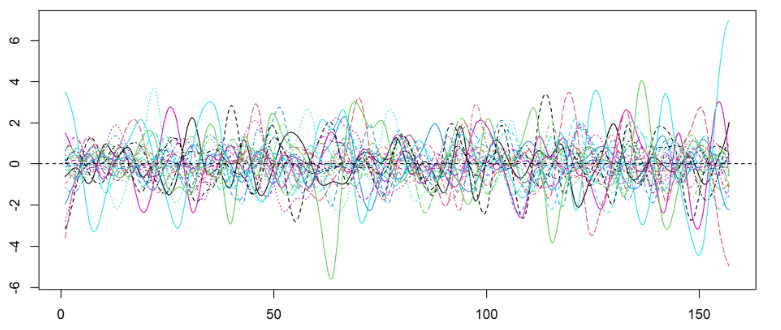
\includegraphics[width=\linewidth]{Figures/After_expansion.png}
         \captionsetup{font=small} % 캡션의 글자 크기를 작게 설정
         \captionof{figure}{BOLD Signals}
    \end{minipage}
    \hfill
    \begin{minipage}{0.14\linewidth}
        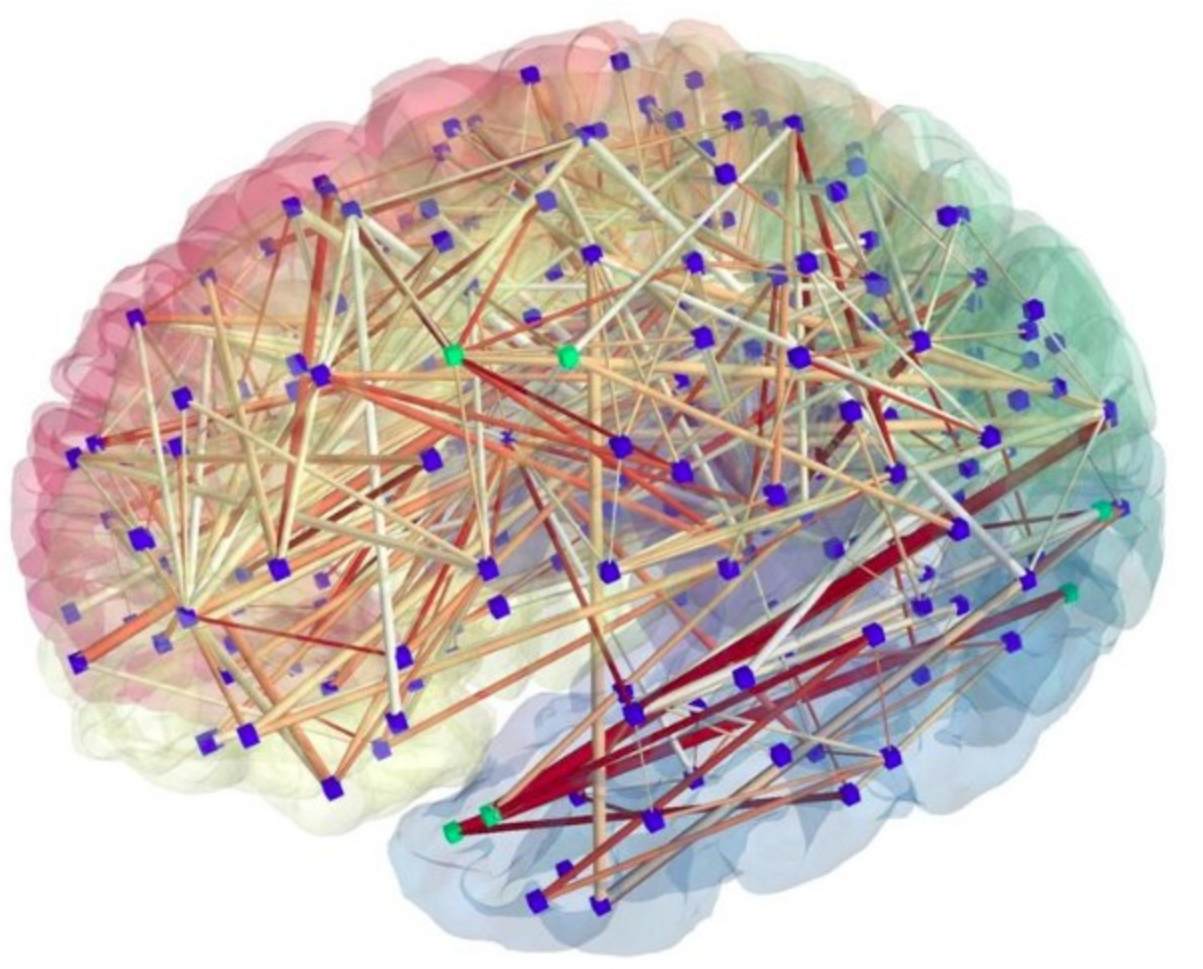
\includegraphics[width=\linewidth]{Figures/Functional Connectivity.png}
        \captionsetup{font=small} % 캡션의 글자 크기를 작게 설정
         \captionof{figure}{FC}
        \label{fig:image2}
    \end{minipage}
    \hfill
    \begin{minipage}{0.20\linewidth}
        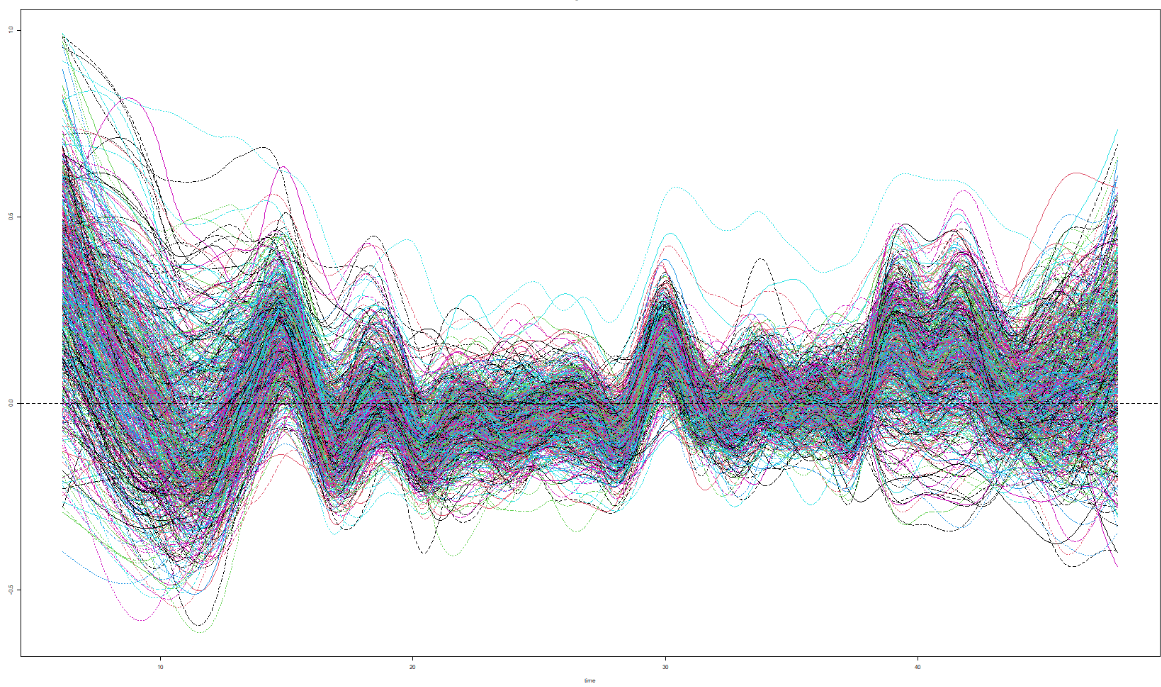
\includegraphics[width=\linewidth]{Figures/FC___FunImgARglobalCWSF___Smoothing.png}
        \captionsetup{font=small} % 캡션의 글자 크기를 작게 설정
         \captionof{figure}{Smoothed FC}
        \label{fig:image3}
    \end{minipage}
    \hfill
    \begin{minipage}{0.38\linewidth}
        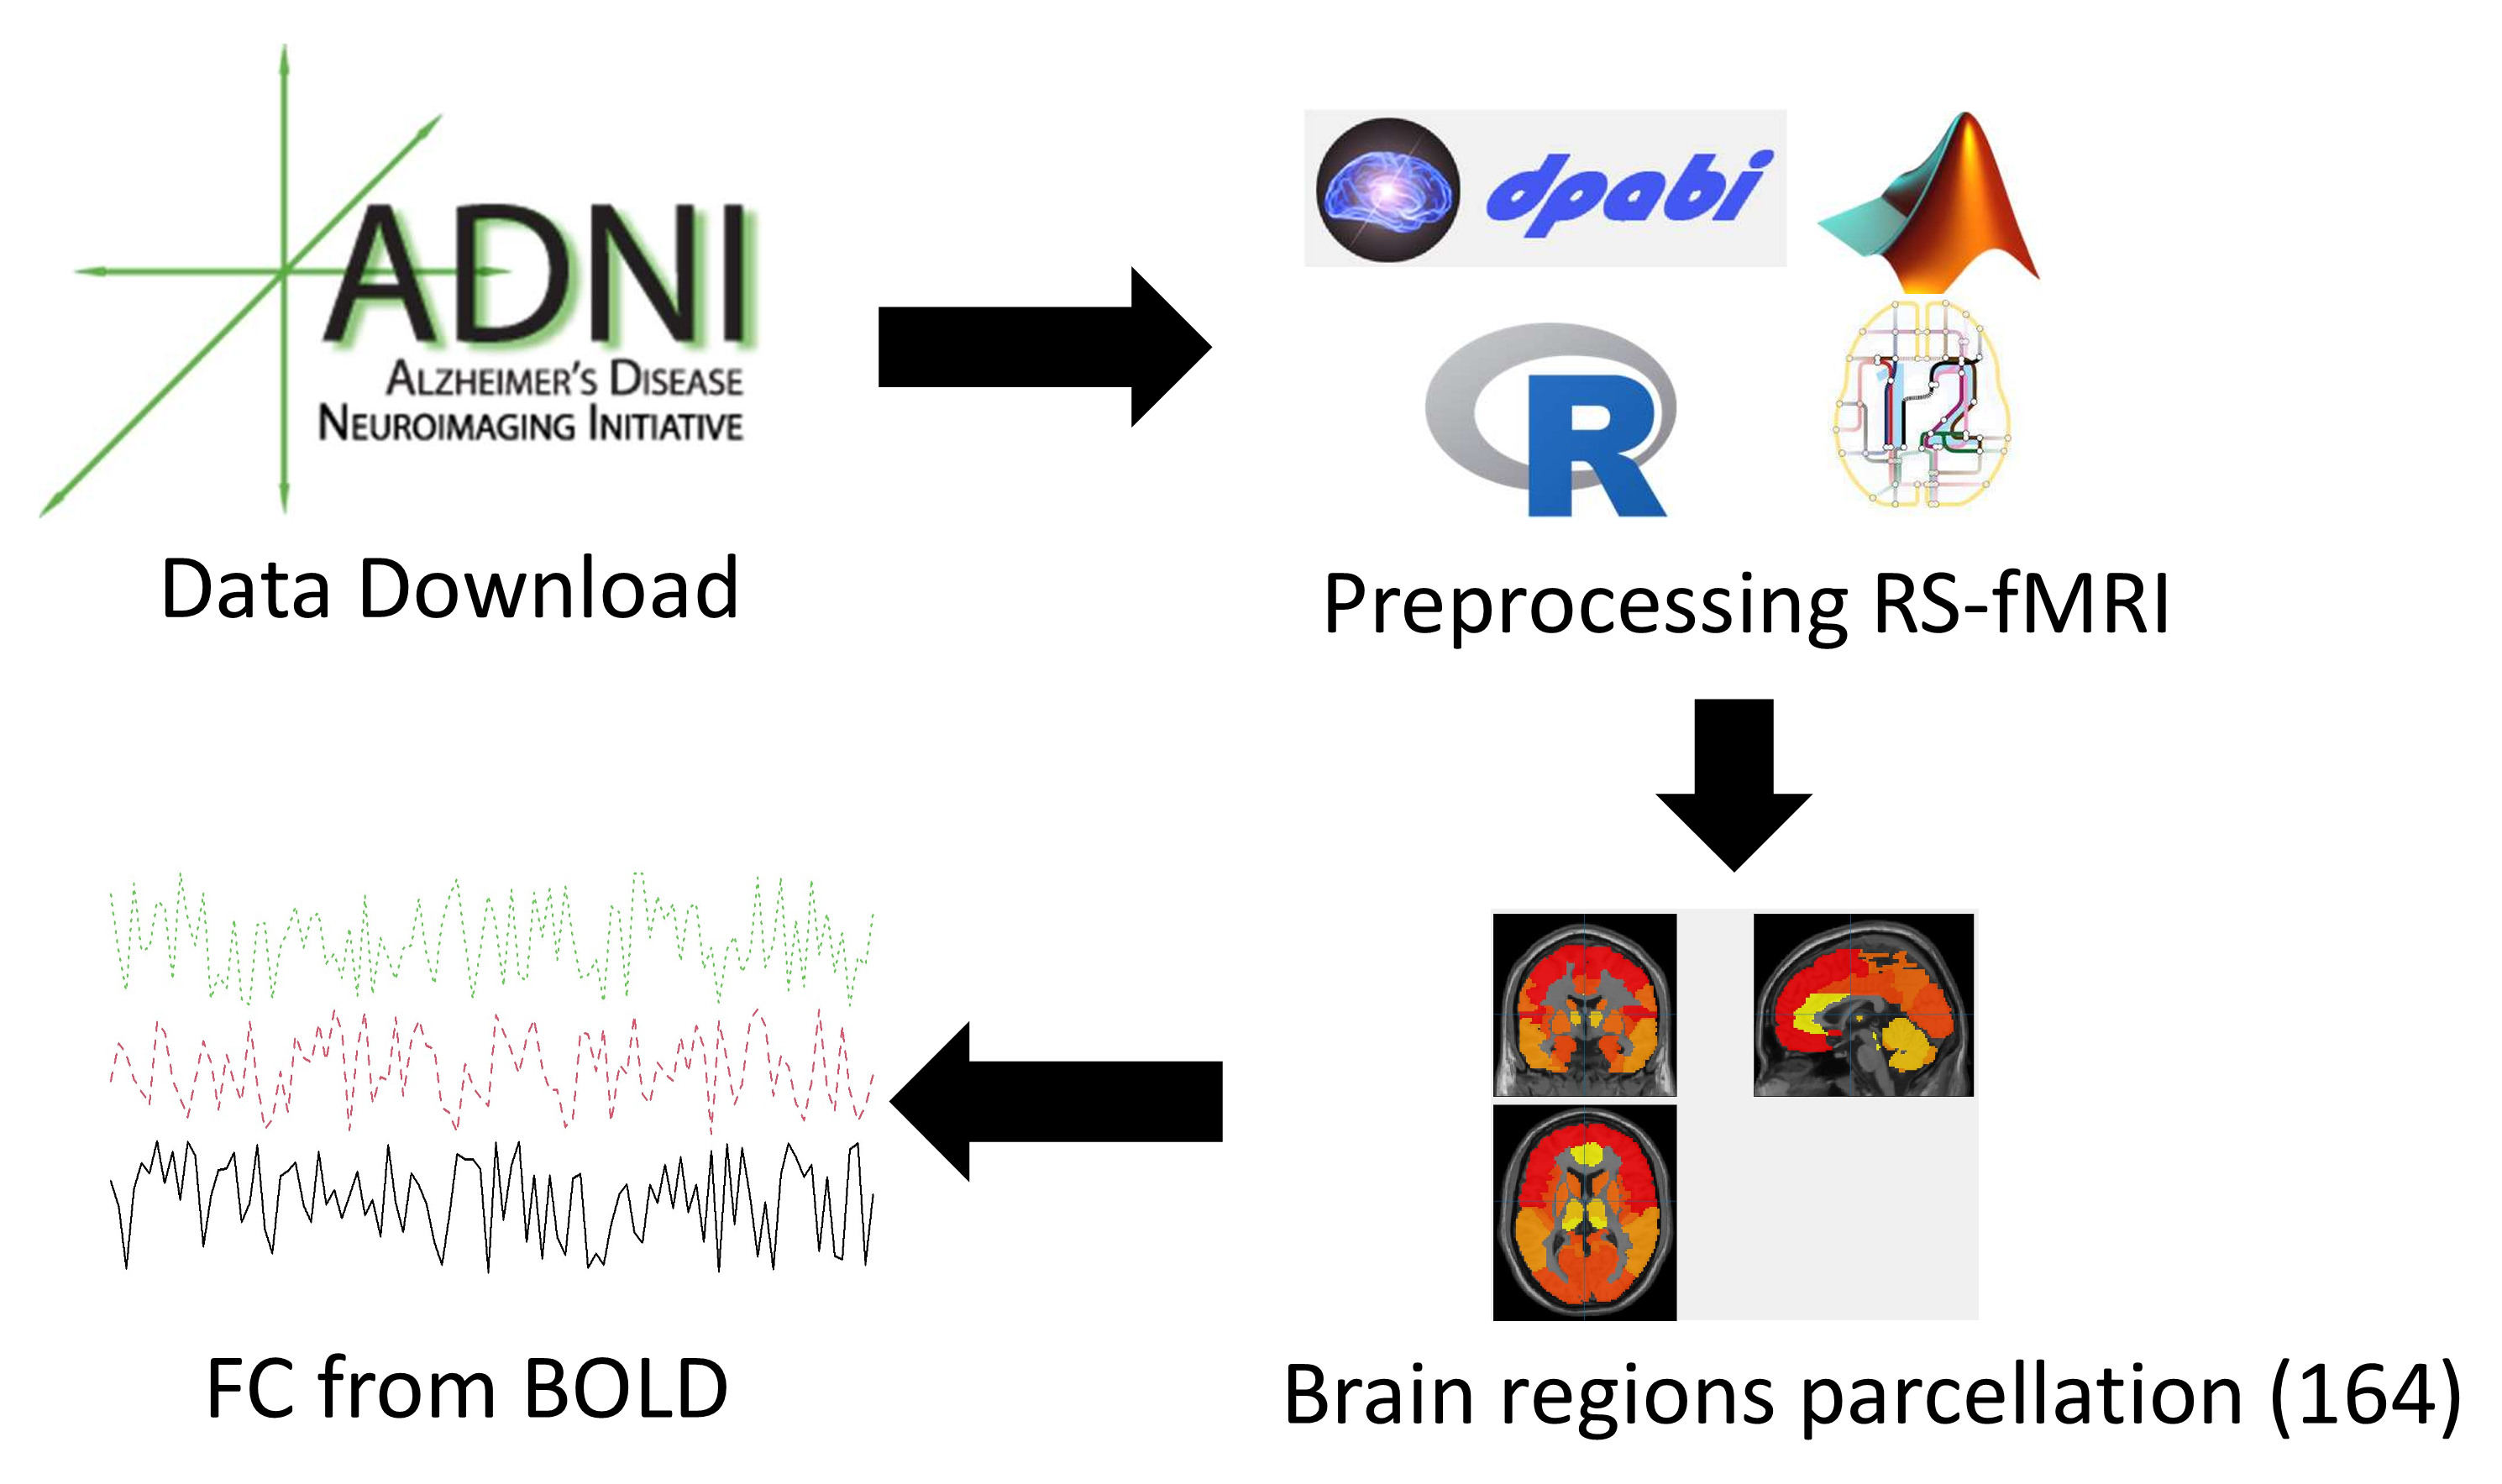
\includegraphics[width=\linewidth]{Figures/Preprocessing_4.png}
        \captionsetup{font=small} % 캡션의 글자 크기를 작게 설정
         \captionof{figure}{Preprocessing}
        \label{fig:image4}
    \end{minipage}
\end{figure}



    
%     \begin{figure}[ht]
%         \centering
%         \begin{minipage}{0.32\linewidth}
%             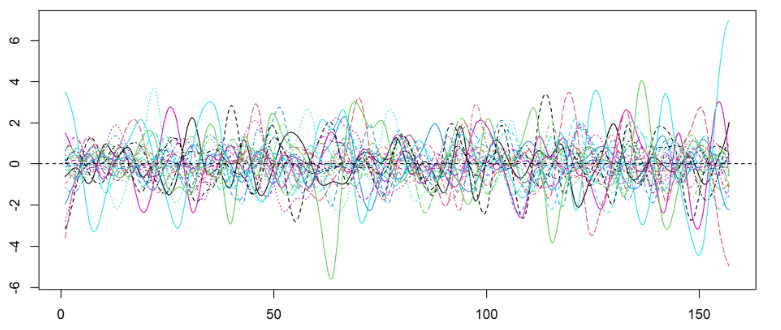
\includegraphics[width=\linewidth]{Figures/After_expansion.png}
%             \caption{Smoothed BOLD Signals}
%             \label{fig:image1}
%         \end{minipage}
%         \hfill
%         %=========================
%         \begin{minipage}{0.32\linewidth}
%             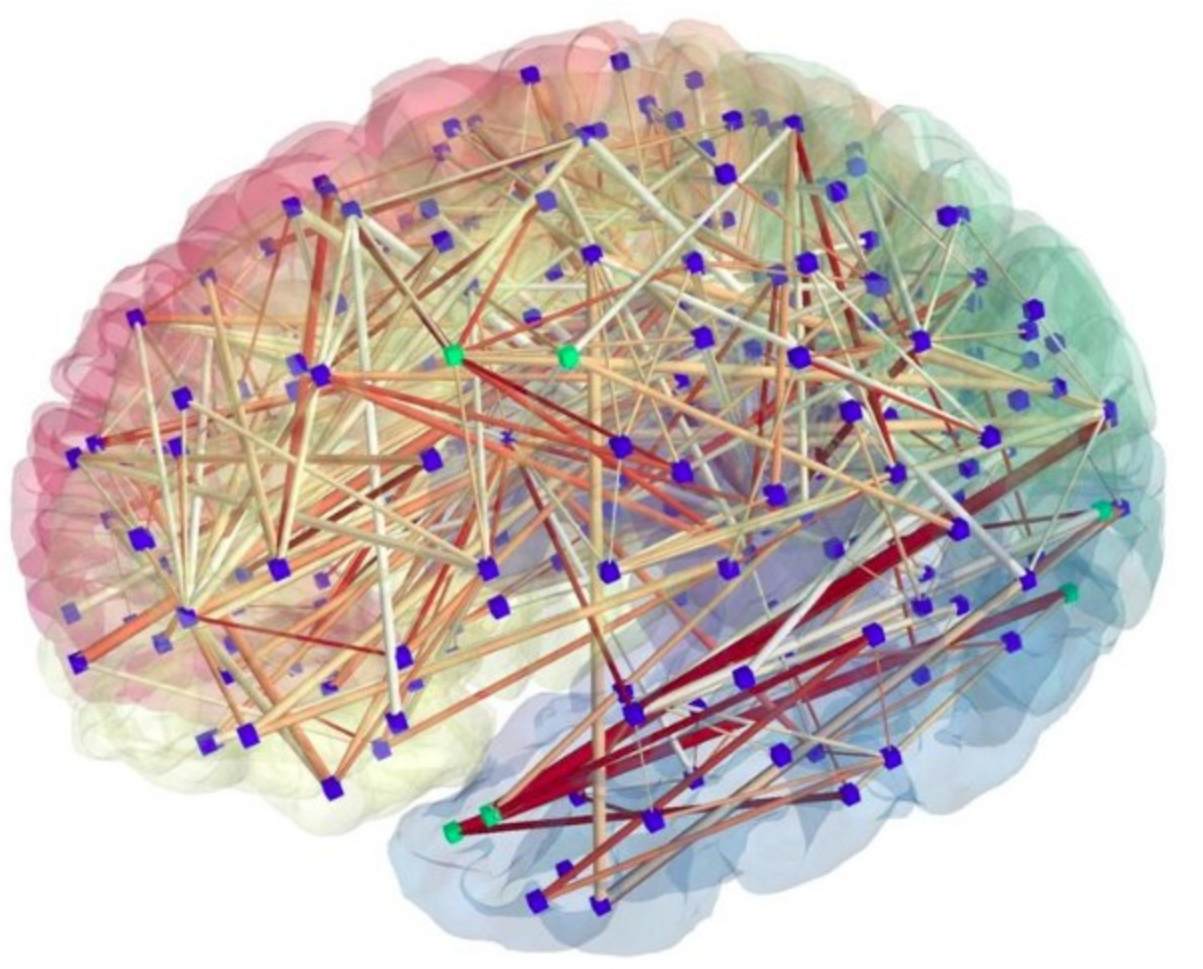
\includegraphics[width=\linewidth]{Figures/Functional Connectivity.png}
%             \caption{Functional Connectivity}
%             \label{fig:image2}
%         \end{minipage}
%         \hfill
%         %==========================
%         \begin{minipage}{0.32\linewidth}
%             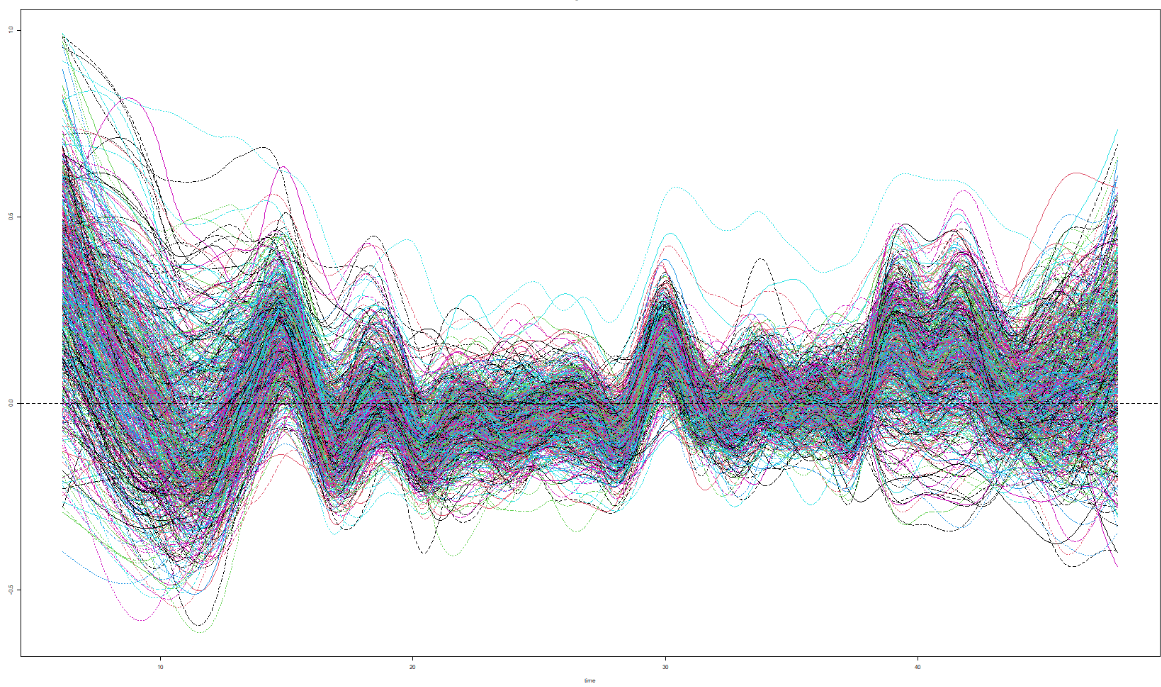
\includegraphics[width=\linewidth]{Figures/FC___FunImgARglobalCWSF___Smoothing.png}
%             \caption{Smoothed FC Signals}
%             \label{fig:image2}
%         \end{minipage}
%     \end{figure}

%     \begin{figure}[ht]
%   \centering
%   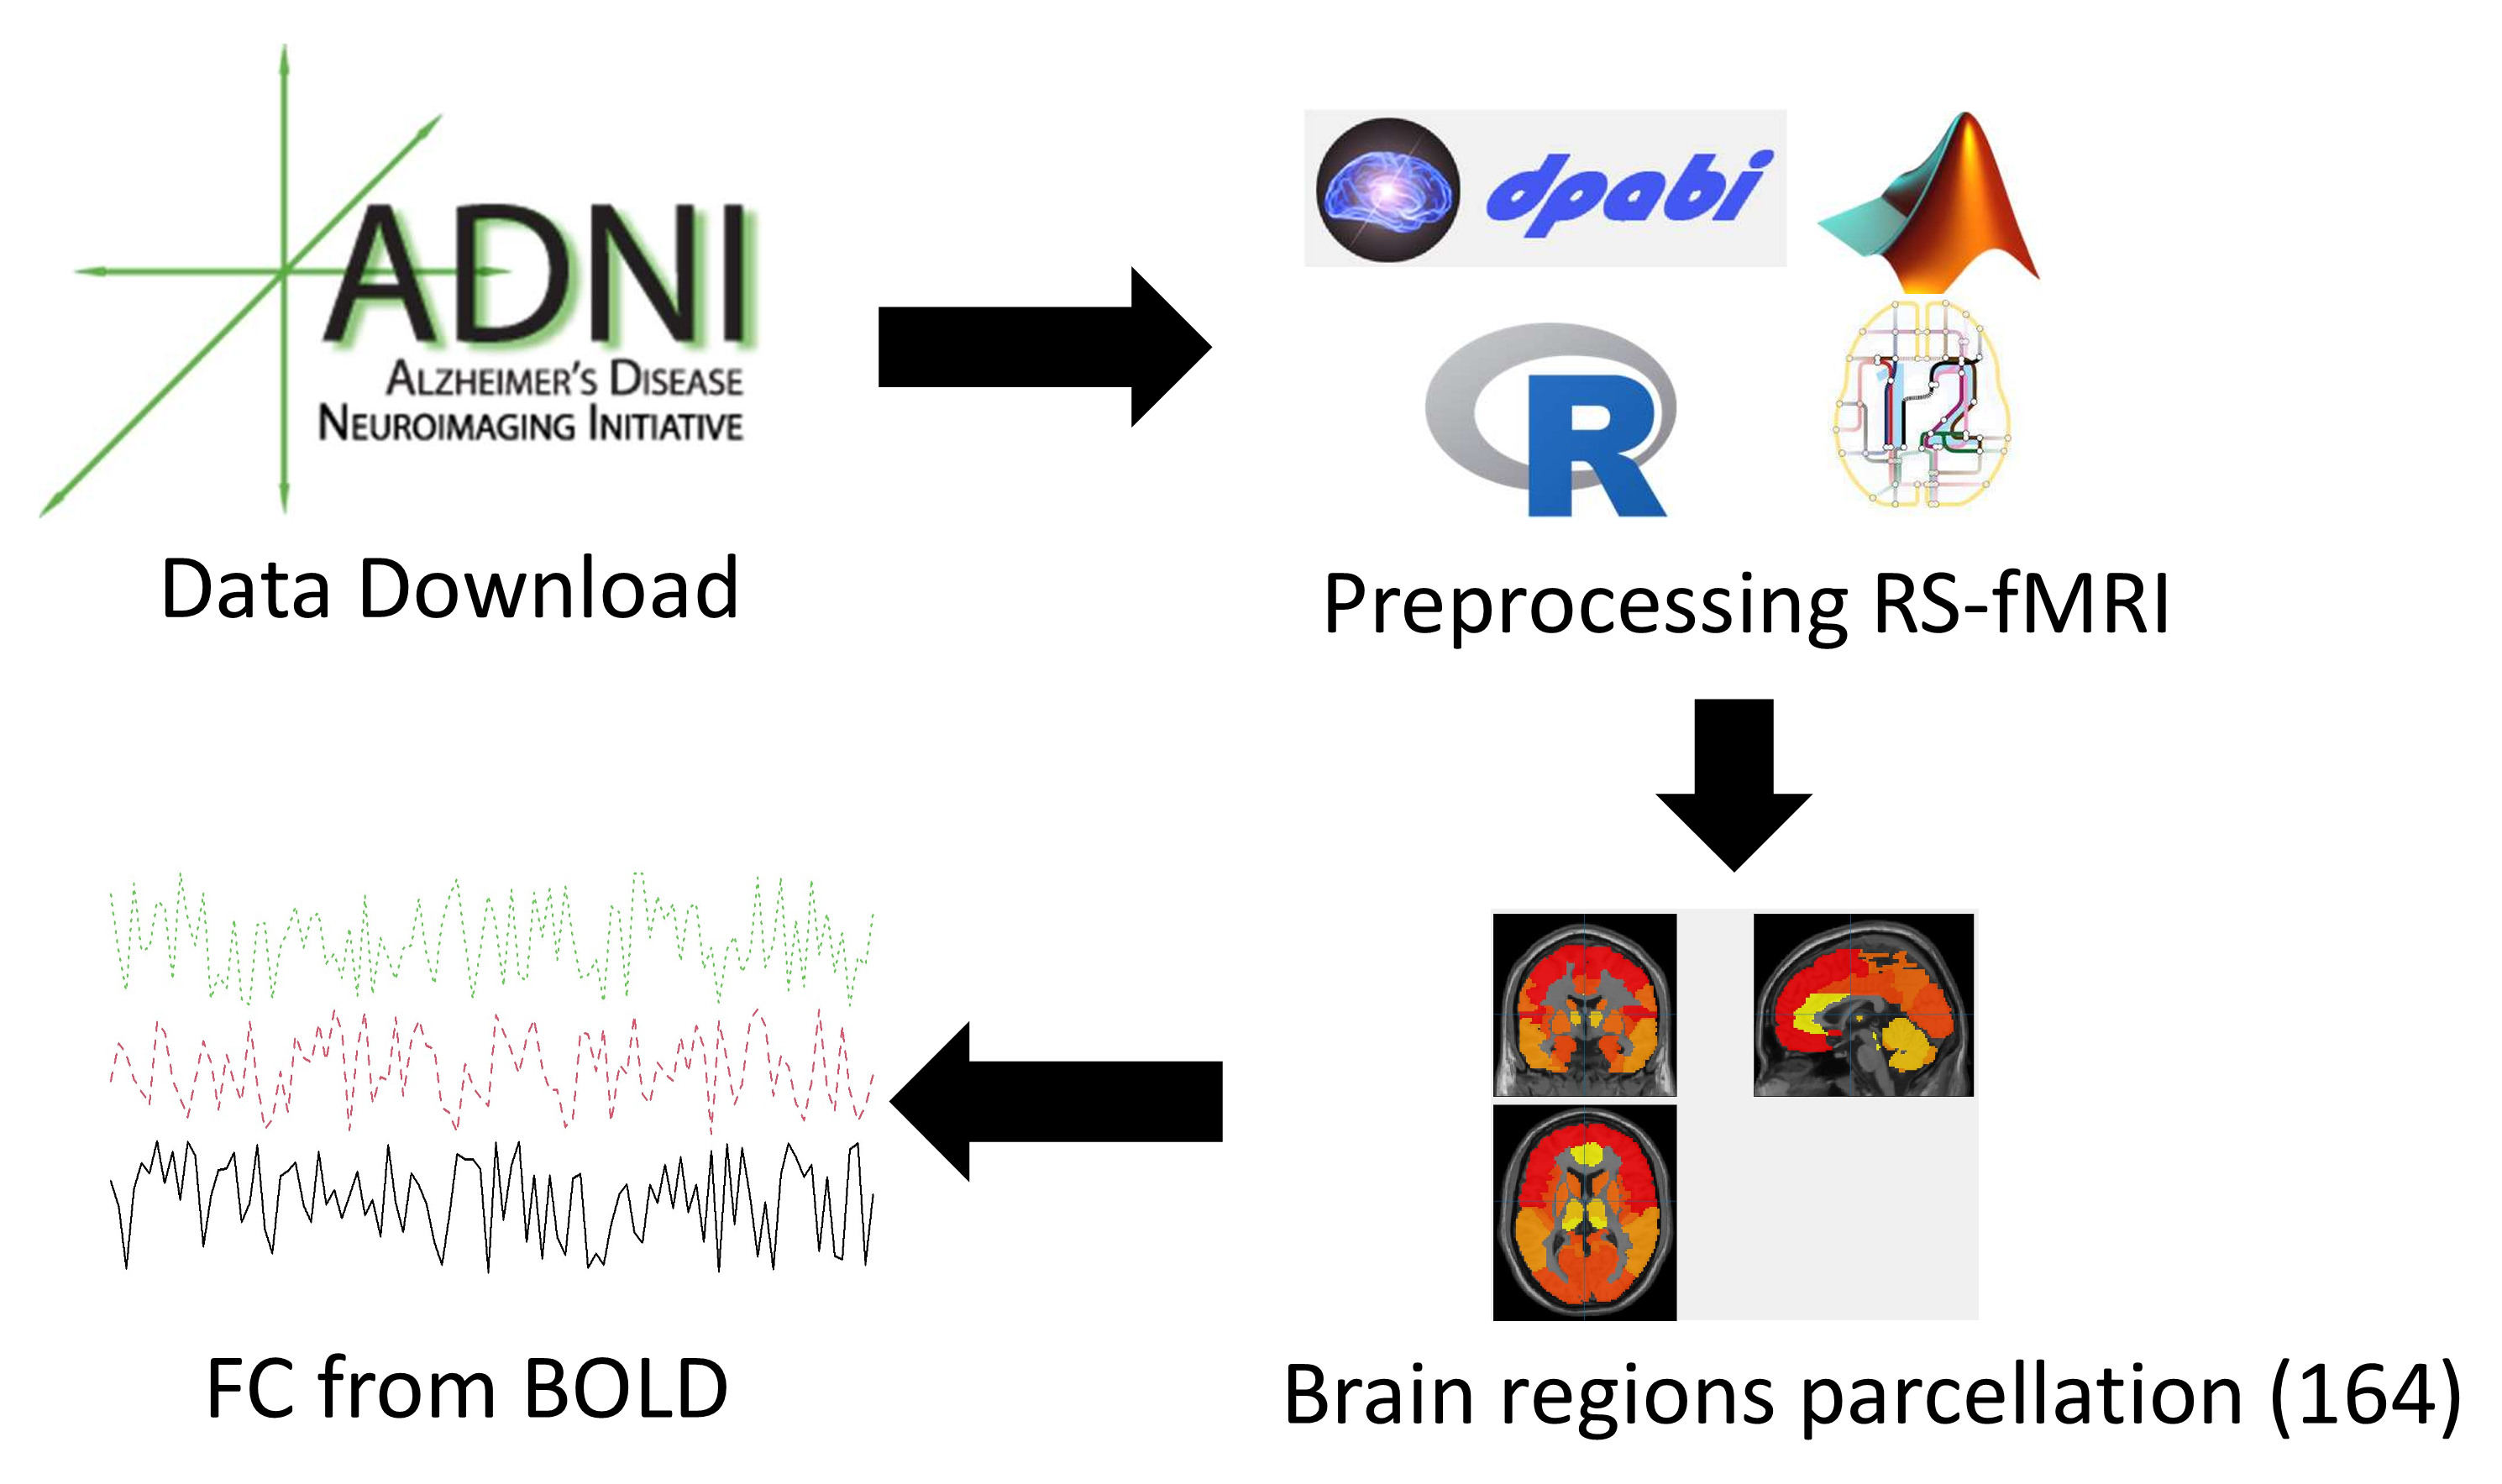
\includegraphics[width=0.5\linewidth]{Figures/Preprocessing_4.png}
%   \caption{Preprocessing}
%   \label{fig:myimage}
% \end{figure}

    
        \begin{itemize}
            \item Since it is difficult to capture internal variation among BOLD signals, it is difficult to apply functional PCA.

            \item From those BOLD signals, Functional Connectivity (FC) can be obtained by Pearson correlation.
        
            \item By brain distances, FCs can be sorted from one brain region, and this can be considered to be functional data.

            \item \textbf{B-spline basis expansion} can be applied to them.
            
        \end{itemize}
    
            \begin{equation*}
                f(t) \approx \sum_{j=1}^{J} c_j \phi_j(t)
            \end{equation*}

            \begin{itemize}
                \item \textbf{Functional PCA (FPCA)} was applied for each functional data from a brain region to extract features.
            \end{itemize}


     \begin{equation*}
         {{\rho }_{\xi }}\left( {{x}_{i}} \right)=\int{\xi \left( t \right){{x}_{i}}\left( t \right)dt}
     \end{equation*}

